\documentclass[12pt]{article}
\usepackage{bbm}
\usepackage{fancyhdr}
\usepackage{titling}
\usepackage{enumitem}
\usepackage{amsmath}
\usepackage{dsfont}
\usepackage{amsfonts}
\usepackage{amssymb}
\usepackage{amsthm}
\usepackage{geometry}
\usepackage{tikz}
\usepackage{algorithm}
\usepackage{algpseudocode}
\geometry{verbose,tmargin=1in,bmargin=1in,lmargin=1in,rmargin=1in}
\renewcommand{\vec}[1]{\mathbf{#1}}
\newcommand{\dec}{\text{dec}}
\newcommand{\divi}{\mathbin{\textnormal{div}}}
\title{Homework 1}
\author{Satvik Prasad}
\date{}
\newtheorem{lemma}{Lemma}[section]
\fancypagestyle{plain}{%
  \fancyhf{}
  \fancyhead[L]{\theauthor}
  \fancyhead[R]{\thedate}
}
\pagestyle{plain}
\makeatletter
\def\@maketitle{%
  \newpage
  \null
  \vskip 1em%
  \begin{center}%
    \let \footnote \thanks
    {\LARGE \@title \par}%
    \vskip 1em%
  \end{center}%
  \par
\vskip 1em}
\makeatother
\usepackage{cmbright}

\newcommand{\mat}[1]{\mathbf{#1}}

% ---------- Probability theory ----------
% Core operators (optional argument-free; use as \E{X}, \Var{X}, \Cov{X}{Y})
\DeclareMathOperator{\EOp}{\mathbb{E}}
\DeclareMathOperator{\VarOp}{Var}
\DeclareMathOperator{\CovOp}{Cov}
\DeclareMathOperator{\CorrOp}{Corr}

\renewcommand{\P}[1]{\mathbb{P}\left(#1\right)}        % \P{A}
\newcommand{\E}[1]{\EOp\left[#1\right]}                % \E{X}
\newcommand{\Var}[1]{\VarOp\left(#1\right)}            % \Var{X}
\newcommand{\Cov}[2]{\CovOp\left(#1,\,#2\right)}       % \Cov{X}{Y}
\newcommand{\Corr}[2]{\CorrOp\left(#1,\,#2\right)}     % \Corr{X}{Y}
\newcommand{\SD}[1]{\operatorname{SD}\left(#1\right)}  % \SD{X}

% Subscripted versions, e.g. \Esub{\theta}{X}, \Psub{\theta}{A}
\newcommand{\Esub}[2]{\EOp_{#1}\left[#2\right]}
\newcommand{\Psub}[2]{\mathbb{P}_{#1}\left(#2\right)}

% Conditioning, indicators, independence
\newcommand{\given}{\,\middle|\,}                      % \E{X \given Y}
\newcommand{\ind}[1]{\mathbbm{1}\left\{#1\right\}}     % \ind{X > 0}
\newcommand{\indep}{\perp\!\!\!\perp}                  % X \indep Y
\newcommand{\iid}{\overset{\text{iid}}{\sim}}          % X_i \iid \Normal(0,1)

% Convergence
\newcommand{\convp}{\xrightarrow{\;p\;}}               % in probability
\newcommand{\convd}{\xrightarrow{\;d\;}}               % in distribution
\newcommand{\convas}{\xrightarrow{\text{a.s.}}}        % almost surely
\newcommand{\convLp}[1]{\xrightarrow{L^{#1}}}          % in L^p

% Probability spaces
\newcommand{\F}{\mathcal{F}}                           % sigma-algebra
\newcommand{\B}{\mathcal{B}}                           % Borel sigma-algebra
\newcommand{\pspace}{(\Omega, \F, \mathbb{P})}

% Common distributions
\newcommand{\Normal}{\mathcal{N}}
\newcommand{\Bern}{\operatorname{Bernoulli}}
\newcommand{\Bin}{\operatorname{Binomial}}
\newcommand{\Pois}{\operatorname{Poisson}}
\newcommand{\Unif}{\operatorname{Uniform}}
\newcommand{\Exp}{\operatorname{Exp}}
\newcommand{\Geom}{\operatorname{Geometric}}
\newcommand{\Gam}{\operatorname{Gamma}}
\newcommand{\Beta}{\operatorname{Beta}}

% Number sets
\newcommand{\R}{\mathbb{R}}
\newcommand{\N}{\mathbb{N}}
\newcommand{\Z}{\mathbb{Z}}


\begin{document}
\begin{enumerate}
    \item We have $f(x, y)$ with joint density
    $$
    f(x, y) = \begin{cases}
        \dfrac{1}{2}(x+y)e^{-(x+y)} & x, y > 0 \\
        0 & \text{otherwise}
    \end{cases}.
    $$
    We find density of $Z = X + Y$ using a change of variables map
    $T: \mathbb R^{2} \to \mathbb R^{2}$ defined by 
    $$
    T(x, y) = (x + y, y)
    $$
    with inverse
    $$
    T^{-1}(z, u) = (z - u, u).
    $$
    This map has Jacobian 
    $$
    J = \begin{vmatrix}
    1 & - 1 \\
    0 & 1
    \end{vmatrix} = 1,
    $$
    and thus for random variables $Z = X + Y, U = Y$ we get joint density $g(z, v)$
    $$
        g(z, v) = \begin{cases}
            \dfrac{1}{2}  ze^{-z} &  z - u, u > 0  \\
            0 & \text{otherwise}
        \end{cases}.
    $$
    Finding the marginal, since we have support on $z > u,$ we get 
    $$
        f_Z(z) = \int_{0}^{z} \dfrac{1}{2}z e^{-z} \, du = \dfrac{1}{2}z^{2} e^{-z}
    $$
    when $z > 0,$ and $0$ otherwise.

    \item Since the uniform distribution is continuous, and the Bernoulli distribution is discrete, we work with CDFs.

    We know $$\mathbb P(X + Y \leq z) = \mathbb P(X + 1 \leq z  \mid Y = 1) \mathbb P(Y = 1) + \mathbb P(X \leq z \mid Y = 0) \mathbb P(Y = 0).$$

    Since $X, Y$ are independent, we can drop the conditionals, yielding
    \begin{align*}
    F_Z(z) = \mathbb P(X + Y \leq Z) &= \dfrac{1}{3}F_X(z - 1)  + \dfrac{2}{3} F_X(z) \\
    &= \begin{cases}
        \dfrac{z+2}{6} & -2 < z \leq -1 \\
        \dfrac{z}{4} + \dfrac{5}{12}  & -1 < z \leq 2 \\
        \dfrac{z}{12} + \dfrac{3}{4} & 2 <  z \leq 3 \\
        0 & z \leq -2 \\
        1 & z > 3
    \end{cases}.
    \end{align*}
    Differentiable points have measure 0, so, differentiating at differentiable points yields
    $$
    f_Z(z) = \begin{cases}
         \dfrac{1}{6} & -2 < z < -1\\
         \dfrac{1}{4}&  -2 < z < 2 \\
            \dfrac{1}{12}  & 2 < z < 3 \\
        0 & \text{otherwise}
    \end{cases}.
    $$

    \item The change of variables satisfies map
    $$
    T(x, y) = ((x-y)/ 2, y),
    $$
    and hence has inverse
    $$
    T^{-1}(u, v) = (2u + v, v).
    $$

    Thus, we have Jacobian
    $$
    J = \begin{vmatrix}
        2 & 1 \\
        0 & 1
    \end{vmatrix} = 2.
    $$
    $X, Y$ have support on $x, y > 0,$ meaning $v > 0$ and $v > - 2u$ are our only constraints. Thus, $U, V$ have joint density
    $$
    f_{U, V}(u, v) = \begin{cases}
        \dfrac{1}{2} e^{-(u + v)} & v> \max(0, -2u)  \\
        0 & \text{otherwise}
    \end{cases}.
    $$

    Integrating to find the marginal of $U,$ we get 
    $$
        f_U(u) = \int_{\max(0, -2u)}^{\infty} \dfrac{1}{2} e^{-(u + v)} \, dv.
    $$
    Thus, if $u \geq 0,$ we have
    $$
    f_U(u) = \dfrac{1}{2}e^{-u}\int_{0}^{\infty} e^{-v} \, dv = \dfrac{1}{2}e^{-u} = \dfrac{1}{2}e^{-|u|}.
    $$
    Otherwise, if $u < 0,$ we get
    \begin{align*}
    f_U(u) &= \dfrac{1}{2}e^{-u}\int_{-2u}^{\infty}  e^{-v} \, dv \\ 
    &= \dfrac{1}{2}e^{-u} e^{2u} = \dfrac{1}{2} e^{u} = \dfrac{1}{2}e^{-|u|}.
    \end{align*}

    Hence, regardless our marginal density for $U$ satisfies
    $$
    f_U(u) = \dfrac{1}{2}e^{-|u|}, \qquad u \in \mathbb R.
    $$

    \item \begin{enumerate}
    
    \item We compute the marginal density:
    \begin{align*}
    f_X(x)= \int_{-\infty}^{\infty} f(x, y)\  dy.
    \end{align*}
    At $X = x,$ $Y$ is supported on the interval $[-\sqrt{1-x^2}, \sqrt{1-x^2}],$ meaning we have
    $$
    f_X(x) = \dfrac{2\sqrt{1-x^2}}{\pi}\, \qquad x \in [-1, 1]
    $$
    and $0$ elsewhere.

    \begin{figure}[h]
  \centering
  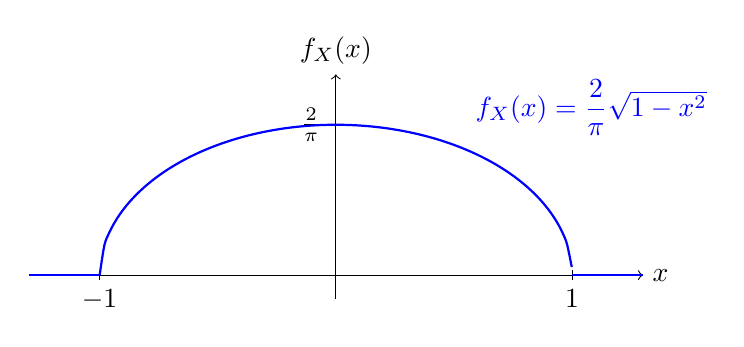
\begin{tikzpicture}[scale=3]
    % axes
    \draw[->] (-1.3,0) -- (1.3,0) node[right] {$x$};
    \draw[->] (0,-0.1) -- (0,0.85) node[above] {$f_X(x)$};

    % tick marks
    \foreach \x in {-1,1} {
      \draw (\x,0.02) -- (\x,-0.02) node[below] {$\x$};
    }
    \draw (0.02,2/pi) -- (-0.02,2/pi) node[left] {$\tfrac{2}{\pi}$};

    % density
    \draw[thick, blue, domain=-1:1, samples=100, smooth]
      plot (\x, {2/pi*sqrt(1-\x*\x)});

    % zero outside the support
    \draw[thick, blue] (-1.3,0) -- (-1,0);
    \draw[thick, blue] (1,0) -- (1.3,0);

    % label
    \node[blue, above right] at (0.55,0.55) {$f_X(x)=\dfrac{2}{\pi}\sqrt{1-x^2}$};
  \end{tikzpicture}
  \caption{Marginal density of $X$ when $(X,Y)$ is uniform on the unit disc.}
\end{figure}

\item The friend is applying the factorization theorem. However, the factorisation theorem requires the factorization to hold over all of $\mathbb R^2,$ but the given factorization is only valid over $D.$ Hence, it can't be applied.

\item Here, the argument would work because we can find such $g, h$ with definition
$$
g(x) = \mathbbm 1_{[-1/2, 1/2]}(x), \qquad \mathbbm 1_{[-1/2, 1/2]}(y)
$$
that factor the density.
\end{enumerate}

\item \begin{enumerate}
    \item We compute $\mathbb E[R]$ using the law of the unconscious statisticiain:
    \begin{align*}
        \mathbb E[R] = \iint_{D} \dfrac{\sqrt{x^2 + y^2}}{\pi} \, dx \, dy.
    \end{align*}

    Using polar coordinates, with the map $T^{-1}(r, \theta) = (r \cos \theta, r \sin \theta),$ and Jacobian
    $$
    J = \begin{vmatrix}
        \cos \theta & -r \sin \theta  \\
        \sin \theta & r \cos \theta
    \end{vmatrix} = r,
    $$
    we get integral
    $$
    \mathbb E[R] = \dfrac{1}\pi{}\int_{0}^{2\pi} \int_{0}^{1} r^2 \, dr \, d\theta = \dfrac{1}{\pi} \int_{0}^{2\pi} \dfrac{1}{3} \, d\theta = \dfrac{2}{3}.
    $$

    \item For $\{R \leq r\},$ we have probability
    $$
    F_R(r) = \dfrac{\pi r^2}{\pi} = r^2,
    $$
    and for $\{R^2 \leq r\},$ we have probability $$
    F_{R^2}(r) = F_{R}(\sqrt{r}) = r.
    $$
    on $r \in [0, 1]$ and $1$ if $r > 1,$ $0$ otherwise.

    \item We compute pdfs via differentiating
    \begin{align*}
        f_R(r) = 2r, \qquad f_{R^2}(r) = 1.
    \end{align*}

    \item \begin{itemize}
        \item We have \begin{align*}
            \mathbb E[R] = \int_{0}^{1} r (2r) \, dr = \dfrac{2}{3}.
        \end{align*}

        \item Alternatively, we have
        $$
        \mathbb E[R] = \int_{0}^{1} \sqrt{r} \cdot 1 \, dr = \dfrac{2}{3}.
        $$
    \end{itemize}
\end{enumerate}
\end{enumerate}
\end{document}